\chapter{Teoretická část}\label{resere}
Tato kapitola obsahuje základní teoretickou informací o technologiích, které jsou použité v současné implementaci aplikace a také o technologiích, které se budou použity při implementaci a analýze.

\section{Pravidla frameworku Angular pro Git}\label{reserse:git}
    Na začátku je potřeba říct, že framework Angular nebude použit v této bakalářské práci. Prozkoumané pravidla nebyly kompletně převzaty, ale byla provedena analýza a následně byly převzaté části, která jsou použitelné při implementaci serveru, který je předmětem teto bakalářské práci. Kompletní přehled pravidel se nachází na GitHub\footnote{ GitHub je webový platformou pro vývoj softwaru pomocí systému řízení verzí Git}\cite{angular-git}.
    
    Pravidla, které byly použity v této bakalářské práce, definují formátování pro \verb|commit| v rámci verzovacího systému Git\footnote{TODO git}. Příčinou zavedení konvenci je potřebnost přidání přehledností dřevu větví. Po dokončeni této bakalářské práci, server bude kompletně funkční, ale proces vývoje se tím neskončí. Budoucí kroky budou podrobně popsány v kapitole \ref{zhodnocení} . Pochopení jednotlivým změnám, udělaným během vývoje softwaru, pomáhají srozumitelné popisy jednotlivých změn. Dosažení takového výsledku působí zavedení jednoho formátu pro každý \verb|commit| v rámci projektu.
    
    \begin{figure}
            \begin{minted}{text}
<type>(<scope>): <subject>
<BLANK LINE>
<body>
<BLANK LINE>
<footer>
            \end{minted}
            \caption{Formát pro \texttt{commit} podle pravidel definovaných pro framework Angular} 
            \label{code:angular-commit}
    \end{figure}
    \begin{figure}
	   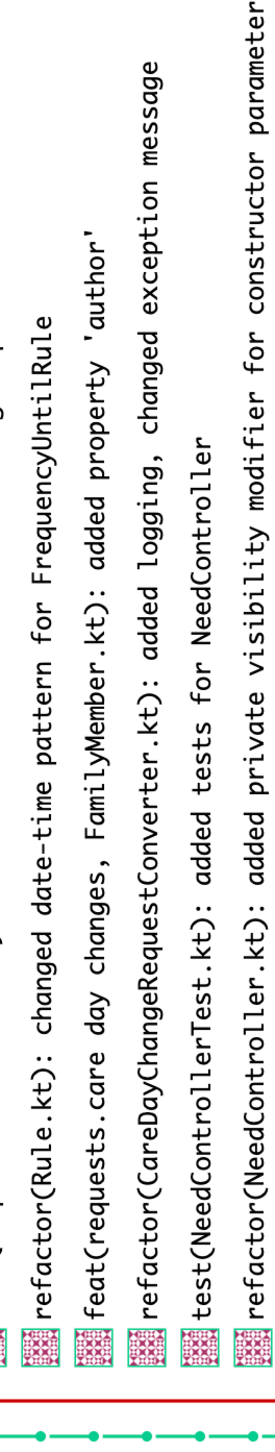
\includegraphics[angle=-90, width=1.0\textwidth]{pdfs/GitLabTree}
	   \caption[Ukázka použití konvenci pro práci z Git]{Ukázka použití konvenci pro práci z Git na grafu větví}\label{image:gitlab-tree}
    \end{figure}
    Tato konvence byla zavedena v moment začátku práci autora na implementaci bakalářské práci (viz obrázek \ref{image:gitlab-tree}). Struktura pro \verb|commit|, která je definovaná ve zdroji (viz obrázek \ref{code:angular-commit}), se skládá ze šestí částí, které byly kompletně převzaty nebo upraveny:
    \begin{itemize}
        \item \texttt{typ}
        \item \texttt{rozsah}
        \item \texttt{předmět}
        \item \texttt{tělo}
        \item \texttt{zápatí}
    \end{itemize}
    
    \subsection{Typ}
        Typ definuje část aplikace, které udělaný \verb|commit| mění. Seznám hodnot, které je možné zadat, je omezený předem definovaným seznamem:
        \begin{itemize}
            \item \texttt{build} -- změny procesu sestavení aplikace nebo úpravy externích závislostí
            \item \texttt{ci} -- změny tykající se průběžné integrace
            \item \texttt{docs} -- změny tykající se jenom dokumentace
            \item \texttt{feta} -- přidání nových funkcí
            \item \texttt{fix} -- oprava chyb
            \item \texttt{perf} -- změny zvyšující efektivitu
            \item \texttt{refactor} -- změny, které nepřidávají nové funkcí a současně neopravují chyby
            \item \texttt{style} -- změny, které nemění význam kódu
            \item \texttt{test} -- přidaní nebo úprava testů
        \end{itemize}
    
    \subsection{Rozsah}
        Rozsah definuje konkretní soubory nebo baličky, které byly změněny. Uvedení rozsah není povinné, ale v rámci této bakalářské práci rozsah bude uveden pro každý \verb|commit|. V případě, že změny byly současně udělaný v několika různých souborech nebo balíčcích, je potřeba uvést je jako seznám oddělený čárkami v kulatých závorkách.
    
    \subsection{Předmět}
        Předmět je stručným popisem udělaných změn. Změny mají být odděleny od typu dvojtečkou. V případě, že \verb|commit| obsahuje několik změn, je potřeba je oddělit čárkou. První písmeno každé změny musí být malé. Poslední změna nekončí tečkou.
    
    \subsection{Tělo}
        Tělo je určeno pro podrobnější popis udělaných změn. Táto část není povinná, ale je doporučena v případě, že udělané změny nejsou pochopitelné po přečtení předmětu nebo není jasná příčina udělané změny.
    
    \subsection{Zápatí}
        Zápatí je určeno pro definování přelomových změn a definování závislostí na konkretní požadavky v rámci GitHub nebo GitLab\footnote{webová platforma pro vývoj softwaru pomocí systému řízení verzí Git}. V rámci této bakalářské práci každému požadavku v rámci GitLab jsou přiděleny jednotlivé větví, proto není potřeba uvádět identifikátor požadavku ve zápatí.
    
\section{Použitý jazyk programování}\label{resere:kotlin}
    Současný návrh aplikace byl proveden v jazyce Kotlin, který je relativně novým jazykem pro JVM\footnote{Java Virtual Machine}. Poprvé tento jazyk byl představen společností JetBrains v 2011 roku. Na moment odevzdání této bakalářské práci byla použita verze 1.3.72 . V porovnání s Java, podpora které je zaručena společností Oracle  a je dlouhodobou a předem definovanou, Kotlin nemá předem definovaný period podpory, ale, podle oficiálních webových stránek zaručuje šeptnou kompatibilitu pro alespoň jednu stabilní verzi, což dovoluje pohodlně migrovat do novější verze jazyku\cite{java-support-period}\cite{kotlin-compatibility}.
    
    %===================================================================
    % Kotlin je relativně nový jazyk pro JVM\footnote{Java Virtual Machine}. Poprvé tento jazyk byl představen společnosti v 2011 roku. První stabilní verze byla představena v únoru roku 2016. Ale už v květnu roku 2017 Kotlin se stal oficiálním jazykem pro Android.
    
    % https://kotlinlang.org/docs/reference/
    Kotlin byl vytvořen jako alternativa jazyku Java a řeší některé jeho problémy. Například, Kotlin řeší problém použití \texttt{null}, také známý jako \texttt{The Billion Dollar Mistake}, a spojené s ním problémy. Java samotna nemá podporu pro \texttt{not-null} proměnné, ale Kotlin takovou podporu má nativně, a to v podobě oddělení \texttt{nullable} typu pomocí ? operátoru. Pro kompletní seznámení s jazykem Kotlin je doporučeno navštívit oficiální webové stránky, kde najdete podrobný návod k použití jazyku\cite{kotlin-documentation}.
    
    % Kotlin je odlišný od Javy i syntaxí. Například není potřeba psát středník pro dokončeni příkazu, ale je vyžadován pouze v případe, že chcete oddělit několik příkazů na jedné řádce. Také byly odstraněny spousta klíčových slov. Například pro deklarací \textit{public final} proměnné je potřeba použit klíčově slovo \textit{val}. Důležitým rozdílem je, že při vytvoření třídy Kotlin umí vygenerovat metody \textit{get} a popřípadě i \textit{set} a umožňuje zadávat defaultní hodnoty v konstruktoru. Také Kotlin zavádí \textit{data class}, který navíc od obyčejné třídy umí vygenerovat metod \textit{toString}, který převádí třídu na typ \textit{String} v čítelné podobě \cite{Priklad vygenerovane tridy}, a metody \textit{equals} a \textit{hashCode}. Celý seznam věcí, které Kotlin má navíc od Javy nebo má jinou implementaci, což není předmětem teto práci, nemá smysl. Proto 
    
    
    % Kotlin je Kotlin podporuje \textit{type-safe builder}

\section{Nástroj pro automatizaci sestavování programu}\label{resere:build}
    % https://gradle.org/maven-vs-gradle/
    % https://www.baeldung.com/ant-maven-gradle
    Pro automatizaci sestavování programu se používá nástroj Gradle, který už se používá v současné implementace aplikace. Existuje populární alternativa -- Maven --, ale Gradle je modernější a pohodlnější. Konfigurace se provádí v jazyce Groove nebo přímo v jazyce Kotlin. Také Gradle poskytuje možnost definovat vlastní úkoly spustitelné pomoci příkazové řádky, které pak budou využité pro analýzu a spuštění testů. Podrobnější informaci o porovnání nástrojů Gradle a Maven lze najit na stránkách \cite{grale-vs-mavem} a \cite{gradle-vs-maven-bealsung}.

\section{Nástroj pro vývoj podnikových aplikací}\label{resere:j2ee}
    % https://spring.io/projects/spring-framework
    % https://spring.io/projects
    % \cite{spring-framework}
    Spring je jeden z nejznámějších frameworků určených pro vývoj podnikových aplikací. Infrastruktura Spring je velká a komplikovaná. Na moment práce na této bakalářské práci, Spring se skládal ze 24 aktivních projektů\cite{spring-projects}. V rámci této bakalářské práci budou využity současně několik různých projektů, které zajišťují korektní funkčnost různých aspektů serveru. V této sekci budou popsány jenom projekty, které budou následně využity při implementaci. Popis je velice stručným a je uveden za účelem zaručení pochopení čtenářem základů použitých technologii. Pro podrobnější informaci o zmíněných projektech je doporučeno navštíví oficiální webovou stránku\cite{spring-official}
    
    \subsection{Spring framework}
        Spring framework je základem pro ekosystém různých projektů, které budou popsány v následujících sekcích\cite{spring-framework}. Tento nástroj samotný je správcem závislostí (\textit{dependency manajer}). Správování závislostí je reprezenotováno pomocí principu \texttt{Inversion of Control} (IoC), což znamená, že framework Spring je kontejnerem, který je zodpovědný za vytváření objektů a provázaní je mezi sebou. Konfigurace aplikace je reprezentována pomocí rozhraní \texttt{ApplicationContext}.
        
        \begin{figure}
            \begin{minted}{yaml}
spring.profiles.active=dev
            \end{minted}
            \caption{Příklad definování profilu aplikace pomocí proměnné prostředí} 
            \label{code:current-spring-profile}
        \end{figure}
        Pro pohodlnou práci a zvýšení efektivity napsaného kódu Spring má navíc od spravování závislostí spoustu skvělých řešení. Jak už bylo zmíněno, popisovat všechno nemá smysl, ale několik nejdůležitějších věcí není možné opomenout. První funkcí, která bude široce využita při implementaci, se týká proměnných v rámci prostředí aplikace. Tyto proměnné umožňují definovat důležité proměnné pro konfiguraci běhu aplikace zvlášť od jejích využití v kódu. Framework Spring umožňuje využit tyto proměnné přímo v kódu. Implicitním souborem obsahujícím tyto proměnné je soubor \texttt{application.properties}. Pro zavedení různých proměnných pro různé případy použití aplikace je možné definovat několik takových souboru pro každý z profilů. Jedinou věcí, kterou je potřeba udělat, je vytvořit soubor, který bude mít v názvu jméno profilu, kterému patří (\texttt{application-{profile}.properties}). Pro definování který profil má použit aplikace v následujících spouštěních, je potřeba v implicitním souboru zadat potřebný profil jako proměnnou (viz obrázek \ref{code:current-spring-profile}). 
        
        
        \begin{figure}
            \begin{minted}{Kotlin}
@Bean
@ConditionalOnProperty(
        value = ["scheduled.alimonyFactory"],
        matchIfMissing = false,
        havingValue = "true")
fun startAlimonyFactory(): AlimonyFactory {
    logger.info("Schedule job: starting AlimonyFactory")
    return AlimonyFactory(
            alimonySettingRepository,
            alimonyRepository)
}
            \end{minted}
            \caption{Příklad aspektově orientovaného programování v Spring} 
            \label{code:spring-conditional}
        \end{figure}
        Spring framework používá techniku vkládání závislosti (\textit{dependency injection}), což nadává možnost psání kvalitnějšího softwaru, ale Spring poskytuje možnost zlepšit výsledný kód ještě více. Framework Spring také používá paradigma aspektově orientovaného programování (AOP). Tato paradigma má za cíl zvýšit modularitu výsledného softwaru pomocí rozdělení kódu do logických častí, nalezení opakujících se častí, které jsou také nazývané průřezové problémy, a nahrazení opakujícího se kódu. Příkladem AOP je anotace zaměřené na podmíněné spouštění metody v závislosti na výsledku předem definované podmínce v závorkách (viz obrázek \ref{code:spring-conditional}).
    
    \subsection{Spring Boot}
        % https://docs.spring.io/spring-boot/docs/current/reference/html/spring-boot-features.html#boot-features-external-config
        Spring Boot je pomocný nástroj pro programátora při konfiguraci aplikace využívající framework Spring. Spring Boot registruje 17 různých implicitních zdrojů proměnných. Kompletní popis zdrojů je na oficiálních stránkách dokumentace\cite{spring-property-sources}. Podle nalezených proměnných framework provádí analýzu konfigurace aplikace a následně, pomocí anotací pro podmínky, automaticky nastavuje prostředí aplikace. Navíc od klasického frameworku Spring, Sping Boot obsahuje rozšířený seznam anotací pro podmínky, které jsou široce využity pro zmíněnou automatickou konfiguraci.\cite{spring-boot}
    
    \subsection{Spring Security}
        Spring Security je framework určený pro návrh autentizace, autorizace a filtrů. Framework vyžaduje využiti frameworku Spring, případně i frameworku Spring Boot. Podrobnou informaci lze najít na oficiálních stránkách\cite{spring-security}.
    
    \subsection{Spring Data}
        Spring Data je framework pro pohodlnou práci programátora při implementaci perzistentní vrstvy\footnote{vrstva aplikace, která komunikuje z databází}. Framewok vytváří dodatečnou vrstvu nad implementací Java Persistense API\footnote{Application programming interface} (JPA). Implementací JPA může být EclipseLink nebo Hibernate. Příkladem využití je rozhraní \texttt{CrudRepository}, které bude využité v této bakalářské práci. Rozhraní definuje základní operace s databází a dovoluje programátorovi jenom definovat typ entity a typ primárního klíče. V případě, že programátor potřebuje složitější dotazy na databází, framework poskytuje možnost definování metod, které ve svých názvech obsahují popis dotazů. Framework rozebírá název na jednotlivé části a překládá ho na SQL\footnote{Structured Query Language} dotaz.
    
    \subsection{Spring Web Services}
        Spring Web Services je framework určený pro implementaci webových služeb. V rámci této bakalářské práci framework bude využit pro implementaci aplikační vrstvy serveru. Aplikační vrstva aplikace má pokrývat případy využití aplikace. Podrobnou informaci lze najít na oficiálních stránkách\cite{spring-web-services}.
        

%  \section{Spring Boot}\label{reserse:spring-boot}
    % https://spring.io/projects/spring-boot
    % \cite{spring-boot}
    % TODO Spring Boot je nástrojem určeným pro rychlý a
    
\section{Testování}\label{resere:testovani}
    Testování aplikace se skládá z několika častí. První část je testování softwaru samotného pro ověření jestli jednotlivé metody, třídy nebo cele moduly fungují správně a komunikují mezi sebou bezchybné. Druhou častí testování je ověření jestli testy pokrývají dostatečnou část kódu a jestli pokrývají důležité funkcí. V této sekci jsou popsány nástroje pro zaručení kvalitního testování, které budou následně využité při implementaci testů a jejích analýze.
    
    \subsection{Spring}
        Framework Spring poskytuje velký počet nástrojů pro testování softwaru. Každý z dodatečných frameworků, jako Súring Boot nebo Spring Security, spolu s novými funkcemi, přidávají vhodné nástroje pro kvalitní testování těchto funkcí. Celý přehled nástrojů, které poskytuje framework, je na oficiálních stránkách dokumentace\cite{spring-tests-doc}. V této sekci jsou uvedeny jenom nejdůležitější použité nástroje.
        
        Prvním nástrojem je anotace \texttt{SpringBootTest}, kterou poskytuje framework Spring Boot pro implementaci integračních testů. Při použití této anotace framework vytvoří nutný kontext aplikace pro kompletní testování.
        
        Druhým důležitým nástrojem je třída \texttt{MockMvc}, která poskytuje možnost kvalitního testování aplikačně vrstvy serveru. Tento nástroj je součásti frameworku Spring Web Services.
        
    \subsection{JUnit}
        JUnit je framework určený pro testování softwaru. V této bakalářské práci bude použita verze 5. Tento framework bude použit pro vytvoření kostry testování. Podrobnější informace o funkcích frameworku je dostupná na oficiálních webových stránkách\cite{junit-doc}.
        
    \subsection{JaCoCo}\label{resere:testovani:jacoco}
         %https://www.jacoco.org/jacoco/trunk/doc/implementation.html
        JaCoCo je nástroj poskytující podrobnou analýzu testů. Tento nástroj bude použit pro výslednou analýzu implementovaných testů a také jako pomocný nástroj pro nalezení důležitých neotestovaných funkcí během implementaci testů. Nástroj existuje v reprezentaci přídavného modulu pro nástroj Gradle, který již se používá v současné implementace programu. Výsledky práci jsou následně uloženy do předem definované složky a jsou reprezentovány pomoci HTML\footnote{Hypertext Markup Language} stránek. Nástroj je otevřeným softwarem, proto podrobnou informaci o implementaci lze najít na oficiálních stránkách\cite{jacoco-implementation}. Výsledky analýzy podle JaCoCo jsou dostupné v příloze \ref{dodatek:code-coverage}.
        
    \subsection{IntelliJ IDEA}\label{resere:testovani:intellij-idea}
        % https://www.jetbrains.com/help/idea/code-coverage.html
        % TODO nastroj pro analyzu pokryti kodu testy \cite{intellij-idea-code-coverage}
        Pro provedení analýzy testů také bylo využité vývojové prostředí IntelliJ IDEA, používané autorem této práci pro implementaci programu. Nástroj pro pokrytí kódu testy je implicitním nástrojem zmíněného vývojového prostředí a poskytuje možnost zobrazování výsledků analýzy přímo v kódu. Takový přístup zrychluje proces implementaci testů. Nástroj také dovoluje vygenerovat výsledky zvlášť od kódu, proto tyto výsledky také jsou dostupné v příloze \ref{dodatek:code-coverage}.


\section{Dokumentace}\label{resere:dokumentace}
    Pro dokumentace API v současné implementace aplikace se používá framework Swagger. Důležitou funkcí, kterou poskytuje framework, je automatické generování dokumentace na základě přidaných anotací v kódu. Dokumentace je následně dostupna z internetu ze stejného adresy jako i server, ale na jiném portu. Podrobná informace o framewoku je dostupná na oficiálních webových stránkách\cite{swagger-doc}.
    
\section{Použité databáze}\label{resere:databaze}

    \subsection{H2}
        % Pro proces vývoje a testování byla zvolena databáze H2\cite{h2-db}, která je relační databází. 
        % http://www.h2database.com/html/tutorial.html
        Současná implementace používá relační databáze H2. Hlavním důvodem zvolení právě této databáze je možnost zvolení několika různých režimu, kde jeden z režimu je vestavěný režim. Tento režim umožňuje usnadnit programátoru práci s databázi, protože se databáze vytváří při spuštění programů a zaniká při její zastavení. Soubory s daty jsou uloženy na disku nebo přímo v paměti. Také H2 má vlastního manažera, který je dostupný přes webový prohlížeč. Podrobnější informace je dostupna na oficiálních webových stránkách\cite{h2-doc}.
        
    \subsection{PostgresSQL}
        % https://www.postgresql.org/docs/12/index.html
        % https://docs.spring.io/spring-cloud-dataflow/docs/1.1.0.RELEASE/reference/html/configuration-rdbms.html
        PostgresSQL je široce využívanou objektově relační databází napsánou v jazyce C. Na moment odevzdání této bakalářské práci je udržovaná PostgreSQL Global Development Group a je otevřeným softwarem. Pro implementaci byla zvolena poslední stabilní verze -- 12. Kompletní dokumentace je dostupná online\cite{postgres-documentation}. Framework Spring, zmíněný v sekci \ref{resere:j2ee}, nativně podporuje použití PostgresSQL\cite{spring-data-postgres}.
        

\section{Nástroj pro analýzu rozsahu implementace}\label{reserse:cloc}
    Nástroj CLOC\footnote{Count Lines of Code}\cite{cloc-download} poskytuje možnost spočítat počet řádek kódu v dáne složce. Nástroj podporuje velký počet jazyku programování. Výsledek obsahuje počet řádek kódu oddělený od komentářů a prázdných řádek. Tento nástroj bude použit pro analýzu současné implementace aplikace a analýzu provedené práce v rámci bakalářské práci.